\subsection{Project 1: ``Price'' of spillover---industry variation in potential for spillover}
\label{sec:rd_potential_for_spillover}

As implied in \Cref{sec:theory_budget_constraint_slope_and_intercept}, when the ``price'' of spillover is high (i.e. it is difficult to obtain spillover due to the host country's absorptive capacity or sector-specific characteristics), the official would choose a bundle that has more private benefits than spillover (\Cref{fig:price_of_spillover}). 

\begin{figure}[!ht]
	\centering
    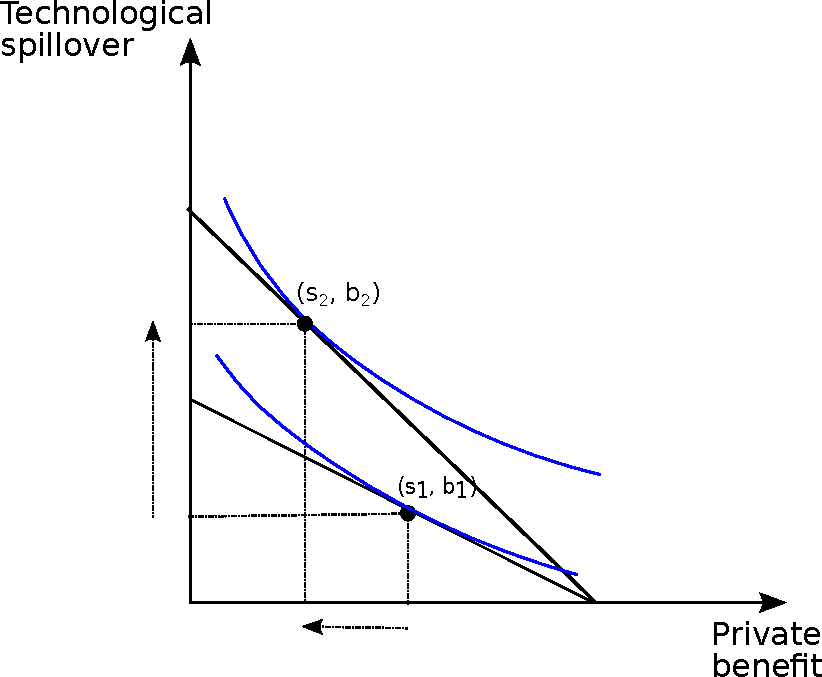
\includegraphics[width=0.75\textwidth, height=0.75\textheight,keepaspectratio]{../figure/price_of_spillover}
    \caption{As the ``price'' of spillover decreases, the official can get a larger amount of spillover given the same budget (i.e. the y-intercept of the budget constraint shifts up). Comparing the bundle $(b_1, s_1)$ and $(b_2, s_2)$, we see that the new bundle has more spillover and fewer bribes.}
    \label{fig:price_of_spillover}
\end{figure}

Here I focus on industry-specific characteristics that either facilitate or hinder spillover.\footnote{Absorptive capacity, or the ability of private firms to learn from their interaction with foreign firms, is also a very important factor in determining spillover. However, given the time-varying nature of absorptive capacity, not to mention the fact that official and domestic firms can strategically invest to improve absorptive capacity, it is much harder to have a research design studying absorptive capacity that claims exogeneity.} Having a divisible production process, manufacturing firms tend to engage more local suppliers and generate more spillover than firms in the primary and tertiary sectors. In addition, within each sector there is a wide variation across industries to be exploited as well. For example, within manufacturing, food processing can have a high level of spillover due to the sourcing of raw materials and packaging. On the other hand, it is harder for foreign firms to work with local suppliers in textile and automotive due the high level of technical sophistication. Similarly, in the service sector, finance, trading, tourism and utilities are generally not divisible into discrete stages to sub-contract. Yet other service industries such as retailing and construction have more opportunities for input suppliers \citep[138]{UNCTAD2001}.

This leads us to the following hypothesis:

\begin{hyp}
Government officials will pursue fewer bribes from firms in industries where it is easier to generate spillover.
\end{hyp}

While such variation across industries is conceptually clear, measurement is thorny given the many factors that can affect the potential for spillover. In addition, there is an endogeneity problem as the potential for spillover may itself be affected by the level of corruption in that industry. For example, an industry plagued by collusive relationship between the official and foreign firms does not offer an enabling environment that allows private firms to develop their absorptive capacity. The endogeneity problem is compounded if the official strategically decides whether to invest and improve absorptive capacity, in which case it is not even clear what is the direction of the bias.

To address both of these measurement and endogeneity issues, I will use the variation in technological spillover across industries in the US as the instrumental variable. The assumption is that the level of technological spillover in a US industry only correlates with the level of bribe in another country's industry through the latent factor that is the industry-specific potential for spillover. The instrument is constructed from US' industries due to the high quality of economic data. Alternatively, for each country, I can use data from a comparable country in the same region or the same developmental stage to construct the instrument.

To measure corruption, presence of FDI, and other firm-level controls, I utilize the World Bank's Enterprise Survey (ES), which includes a wealth of firm-level data across 125 countries, spanning various topics from investment, labor, to business-government relation \citep{WorldBank2015}. The Enterprise Survey uses stratified random sampling (using three strata: firm size, business sector, and region) in order to ensure representativeness. The survey data comes from face-to-face interviews with upper management and is anonymized to ensure confidentiality at all times.\footnote{For more on the methodology of the Enterprise Survey, visit \url{http://www.enterprisesurveys.org/methodology}} This dataset has a wealth of firm-level data that helps us operationalize key concepts as detailed below.

Operationalization of variables:
\begin{itemize}
\item FDI spillover: See \Cref{sec:measure_spillover}. The level of FDI by sectors is available via the Enterprises Survey dataset.\footnote{It would be better if there is UNCTAD data for FDI by sector, since the Enterprize Survey is not designed to account for all FDI inflow. Without weights, it is difficult to accurately get the population of foreign firms from the ES' sample of foreign firms.}

\item Corruption: can be measured in two ways. 1) Firms' perception about corruption as an obstacle. This measure is frequently used but is not accurate since firms' perception of corruption depends not only on the level of corruption but also the characteristics of firms. 2) Hard measure of prevalence and depth of bribes, e.g. ``Was an informal payment expected or request (when applying for a license)?'', ``How much do establishments like this one give in informal payments?'' 
\end{itemize}